
\documentclass[a4paper, 10pt]{article}
\usepackage[spanish]{babel}
\usepackage[utf8]{inputenc}
\usepackage[top=1 in, left=1 in, right=1 in, bot=1 in]{geometry}
\usepackage{amsmath, amsthm, amsfonts}
\usepackage{graphics}
\usepackage{float}
\usepackage{epsfig}
\usepackage{amssymb}
\usepackage{latexsym}
\usepackage{newlfont}
\usepackage{epstopdf}
\usepackage{amsthm}
\usepackage{epsfig}
\usepackage{caption}
\usepackage{multirow}
\usepackage[colorlinks]{hyperref}
\usepackage[x11names,table]{xcolor}
\usepackage{graphics}
\usepackage{wrapfig}
\usepackage[rflt]{floatflt}
\usepackage{multicol}
\usepackage{longtable,multirow,booktabs}
\usepackage{listings} \lstset {language = Python, basicstyle=\bfseries\ttfamily, keywordstyle = \color{blue}, commentstyle = \bf\color{green}, backgroundcolor = \color{gray!5}, stringstyle = \color{yellow!5}}
\usepackage{titlesec}

% \titleformat{\section}{\filcenter}{}{8pt}{}

\setcounter{secnumdepth}{0}

\title{Recuperación del Sistema de Ficheros}
\author{Alexander Antonio González Fertel C-512 \hfill
		\href{mailto:a.fertel@estudiantes.matcom.uh.cu}{a.fertel@estudiantes.matcom.uh.cu}\\
		Hieu Do Ngoc C-511 \hfill
		\href{mailto:a.fertel@estudiantes.matcom.uh.cu}{a.fertel@estudiantes.matcom.uh.cu}\\
		Joel David Hernández Cruz C-511 \hfill
		\href{mailto:j.cruz@estudiantes.matcom.uh.cu}{j.cruz@estudiantes.matcom.uh.cu}}
\date{}

\newtheorem{definition}{Definici\'on}

\begin{document}
	\maketitle
	% \newpage

	\section{Interfaz de Usuario}
	El sistema de recuperación de información implementado consta de una aplicación de escritorio como medio de comunicación con los modelos
	de recuperación de información implementados. Como se puede ver en la imagen~\ref{fig:1}, en la interfaz se presentan 2 zonas de 
	interacción, al inicio (Configuración), se escoge el modelo a usar y se selecciona (provee) un directorio a indexar, los cuales
	se guardan para realizar las consultas a través del botón \textit{Submit}. Debajo se presenta una entrada
	de texto para formular la consulta, lo cual deviene en un ranking de los documentos que se muestra luego al presionar el botón
	de búsqueda.

	\begin{figure}[h]
		\centering
		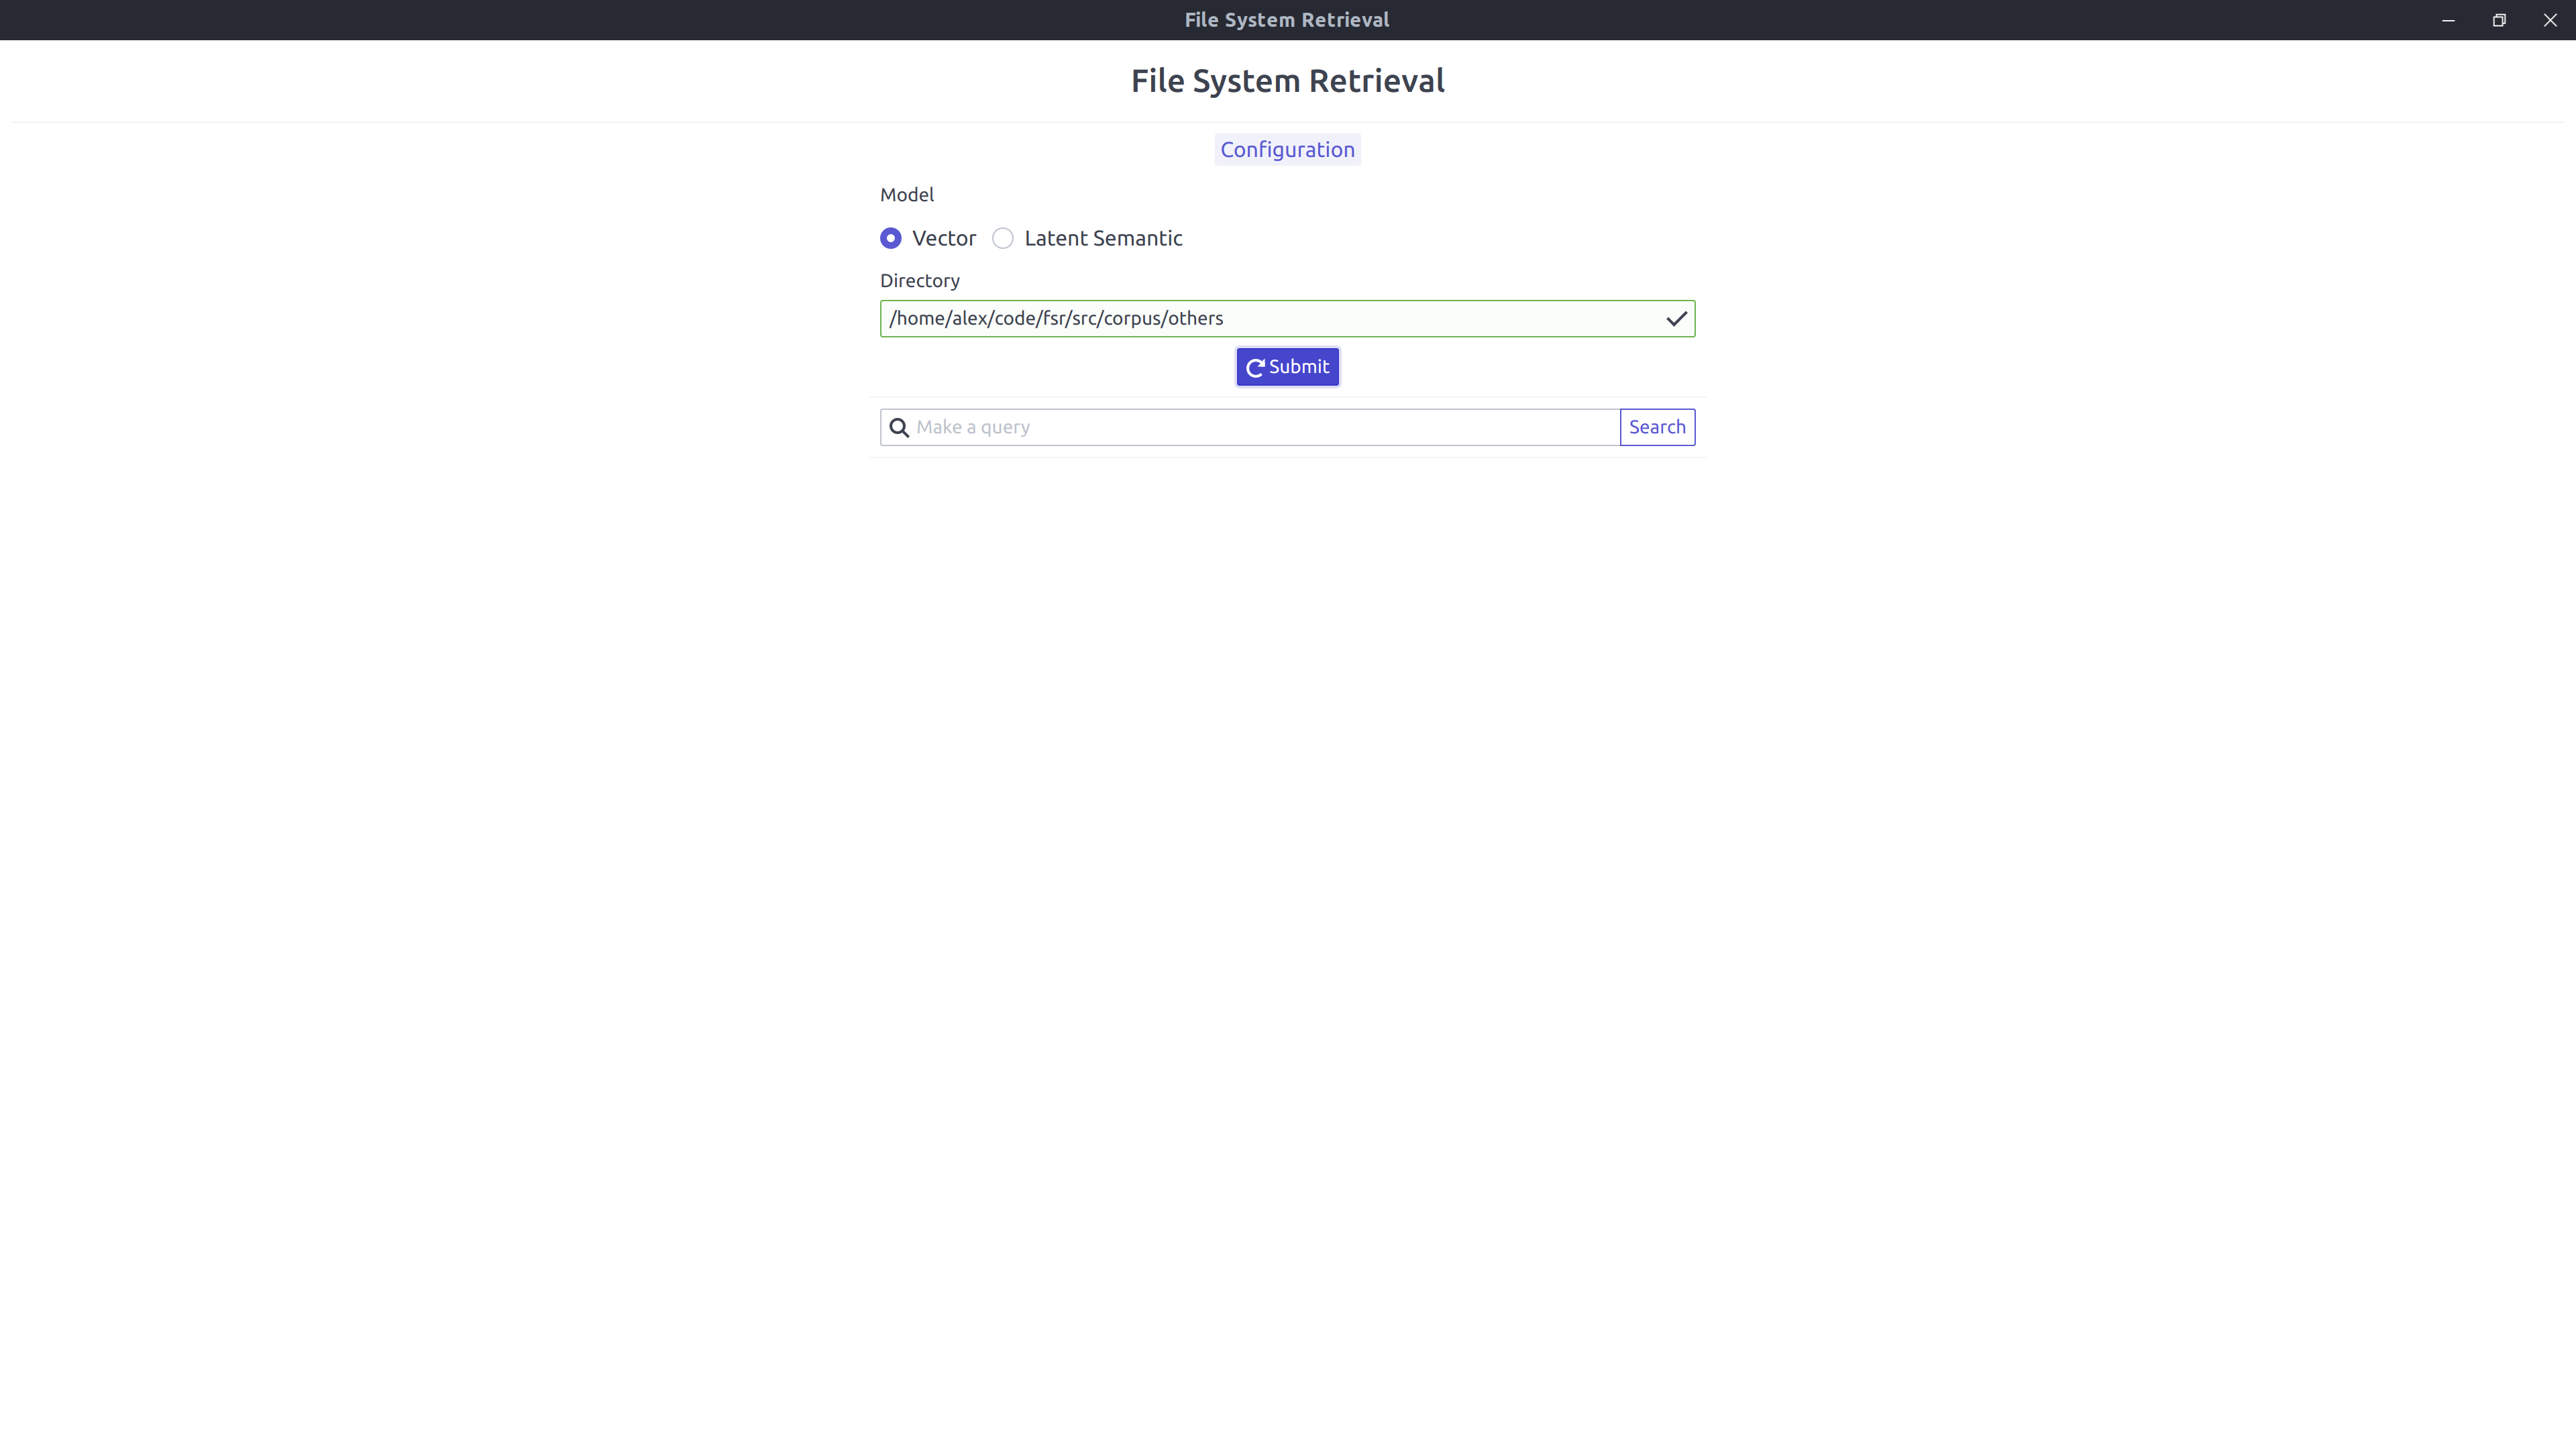
\includegraphics[width=.6\textwidth]{images/app.png}			
		\caption{File System Retrieval}
		\label{fig:1}	
	\end{figure}

	\section{Modelo}
	El principal modelo de recuperaci\'on de informaci\'on implementado en el sistema de recuperaci\'on de informaci\'on es 
	el modelo de Indexaci\'on Sem\'antica Latente (LSI). El modelo LSI es una variación del Modelo Vectorial, en la que los
	documentos se representan a partir de vectores de pesos no binarios, al igual que las consultas, la función de similitud
	es el coseno del ángulo entre el vector del documento y el de la consulta.

	La idea principal de este modelo consiste en hacer un mapa entre cada documento y el vector consulta a un espacio 
	de dimensi\'onalidad reducida el cual est\'a asociado a conceptos.
	
	\begin{definition}
		Sea t la cantidad de t\'erminos \'indice en la colecci\'on y N el total de documentos. Se define $M=(m_{i,j})$ 
		como la matriz de asociaci\'on de t\'ermino-documento con t filas y N columnas. 
		Cada elemento $m_{i, j}$ de la matriz M es el peso asociado a la pareja t\'ermino i - documento j. 
	\end{definition}
	
	Existen diferentes formas de generar estos valores $m_{i,j}$, ya sea usando la frecuencia t\'ermino-documento 
	o usando la matriz de tf-idf. El SRI implementado, elige usar la matriz tf-idf como la matriz de asociaci\'on 
	t\'ermino-documento, al ser esta una de las t\'ecnicas de \textit{"term-weighting"} m\'as populares que existen 
	en la actualidad. Adem\'as, su implementaci\'on resulta bastante sencillo y eficiente haciendo uso de la librer\'ia $scikit-learn$.
	
	Para lograr la reducci\'on de dimensiones de la matriz $M$, el modelo LSI propone utilizar la 
	t\'ecnica de descomposici\'on \textit{SVD} para descomponer la matriz $M$ en 3 componentes de la manera siguiente.

	\begin{equation}
		M = KSD^t
	\end{equation}
	
	La matriz $S$ es una matriz diagonal $r*r$ de valores singulares (ordenados de mayor a menor) donde $r = min(t, N)$ es el rango de la matriz $M$.
	
	Si conservamos s\'olamente los $s$ mayores valores singulares de $S$ y sus correspondientes columnas en $K$ y $D$.
	La matriz resultante es la matriz de rango $r$ que mayor aproxima a la matriz original $M$ usando como m\'etrica la
    norma de \textit{Frobenius}. Esta matriz esta dada por
	
	\begin{equation}		
		M_s = K_sS_sD^t_s
	\end{equation}

	donde $s$, $s < r$, es la dimensión del espacio de conceptos reducidos. La selecci\'on de un valor para $s$ se
	realiza para balancear 2 efectos opuestos. Primero, $s$ debe ser suficientemente grande para representar todas las propiedades
	de los datos reales. Y segundo, $s$ debe ser suficientemente peque\~no para permitir el filtrado de detalles irrelevantes
	en la representaci\'on.

	Para este modelo LSI, utilizamos la librer\'ia $scikit-learn$ para realizar la reducci\'on de dimensionalidad
	de la matriz $M$. La dimensionalidad del espacio de conceptos reducidos esta dado por

	\begin{equation}
		s = min(100, t, N)	
	\end{equation}

	debido a que esta librer\'ia recomienda a sus usuarios utilizar $s = 100$ cuando se trabaja en \'analisis de s\'emantica latente.

	Para rankear los documentos con respecto a una consulta, simplemente se modela la consulta como un 
	\textit{pseudo-documento} en la matriz t\'ermino-documento $M$. Asumiendo que la consulta es el 
	documento n\'umero 0, entonces la primera fila de la matriz $M^tM$ proporciona los valores de similaridad de los documentos
	con respecto a la consulta.

	Adem\'as, la aplicaci\'on provee una implementac\'ion del modelo cl\'asico de espacio vectorial para que
	el usuario pueda realizar comparaciones de los resultados obtenidos por los dos modelos.

	\section{Evaluación}
	Para obtener estos resultados, se escogen 30 consultas ya \textit{tagueadas} sobre un conjunto de 1033 documentos.
	
	A continuación los promedios de precisión, recobrado, f-medida y r-precisión obtenidos, usando un R=10:
	
	\begin{enumerate}
       \item Precisión Promerdio = 0.22
        \item Recobrado Promedio = 0.77
        \item F-medida Promedio = 4.83
        \item F1-medida Promedio = 3.10
        \item R-Precisión Promedio = 0.71

    \end{enumerate}
\end{document}
